\subsection{Potencia Eléctrica}
La potencia eléctrica es una medida de la cantidad de energía que se consume, produce o transfiere en un circuito eléctrico en un período de tiempo determinado. Es un concepto fundamental en el estudio y diseño de sistemas eléctricos y electrónicos. 
Cuando se trata de corriente continua (CC) la potencia eléctrica desarrollada en un cierto instante por un dispositivo de dos terminales, es el producto de la diferencia de potencial entre dichos terminales y la intensidad de corriente que pasa a través del dispositivo. Por esta razón la potencia es proporcional a la corriente y a la tensión

\begin{equation}
    P= V \cdot I 
\end{equation}

En cambio, cuando se trata de corriente alterna (AC) sinusoidal, el promedio de potencia eléctrica desarrollada por un dispositivo de dos terminales es una función de los valores eficaces o valores cuadráticos medios, de la diferencia de potencial entre los terminales y de la intensidad de corriente que pasa a través del dispositivo. 


Existen 3 tipos de potencias presentes en un circuito de CA, la potencia activa, la potencia reactiva y la potencia aparente. La relación entre estas se puede observar a través del llamado triangulo de potencias. 

\begin{figure}[h]
    \centering
    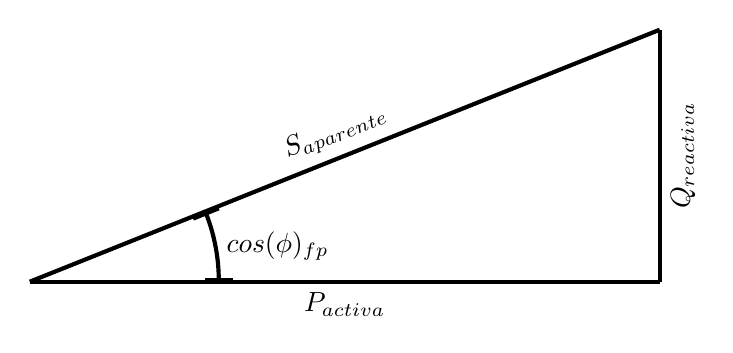
\begin{tikzpicture}[scale=0.8]
    \draw[line width = 1.5pt, black] (0,0)--(10,0) node[midway, below]{$P_{activa}$};
    \draw[line width=1.5pt, black](10,0)--(10,4) node[midway,below,sloped]{$Q_{reactiva}$};
    \draw[line width=1.5pt,black](10,4)--(0,0) node[sloped,midway,above]{$S_{aparente}$};
    \draw[line width=1.5pt,black,|-|](3,0) arc (0:21.8:3) node[midway,right]{$cos(\phi)_{fp}$};
\end{tikzpicture}
    \caption{Triángulo de potencias}
    \label{fig:triang_pot}
\end{figure}
\subsubsection{Potencia activa}
Es la potencia capaz de transformar la energía eléctrica en trabajo. Los diferentes dispositivos eléctricos existentes convierten la energía eléctrica en otras formas de energía tales como: mecánica, lumínica, térmica, química, etc. Esta potencia es, por lo tanto, la realmente consumida por los circuitos y, en consecuencia, cuando se habla de demanda eléctrica, es esta potencia la que se utiliza para determinar dicha demanda. 
Se designa con la letra (\textbf{P}) y se mide en vatios —watt— (W) o kilovatios —kilowatt— (kW).
\begin{equation}
    P=  V\cdot I\cdot\cos \phi
\end{equation}

\subsubsection{Potencia reactiva}
La potencia reactiva es la potencia que fluye entre el equipo eléctrico y la fuente de alimentación debido a la capacitancia o inductancia del equipo. No realiza trabajo útil en el circuito, sino que se intercambia entre la fuente de energía y los dispositivos inductivos o capacitivos. Su efecto principal es el almacenamiento y la liberación de energía magnética.
Se representa con la letra (\textbf{Q}) y Se mide en voltamperios reactivos (VAR).

\begin{equation}
    Q = V\cdot I\cdot\sen \phi
    \label{eq:visenphi}
\end{equation}

\subsubsection{Potencia aparente}
La potencia aparente (\textbf{S)} es la suma vectorial de la potencia activa y la potencia reactiva. Se mide en voltamperios (VA). Representa la magnitud total de la potencia que fluye en un circuito, incluyendo tanto la potencia activa como la reactiva. Es la potencia que se observaría si solo se midieran los voltajes y corrientes en el circuito y si no existiera un desfasaje entre ellos. 
\begin{equation}
    S= V \cdot I
\end{equation}

\subsection{Factor de potencia}
Como ya se explicó, la energía presente en un sistema
de corriente alterna en régimen permanente está compuesta por una parte
que realiza un trabajo y por otra parte que se almacena
en los elementos reactivos y se intercambia con la fuente. La relación que existe entre la energía aprovechada (la que es capaz de realizar un trabajo) y la energía total disponible se conoce como \textit{factor de potencia} ($\mathrm{fp}$). Estas energías se relacionan con la siguiente expresión:

\begin{equation}
    \mathrm{fp} = \frac{P}{S} = \cos(\phi)
\end{equation}

Por su definición, el factor de potencia es el rendimiento del sistema, y
como tal, es un número adimensional comprendido entre 0 y 1. Un factor de potencia cercano a 1 indica que la mayor parte de la energía es utilizada para realizar trabajo.

\label{sec:fp}
\subsubsection{Corrección del factor de potencia}
La energía transportada que no se consume produce pérdidas, sobrecarga los transformadores y por lo tanto disminuye la eficiencia del sistema eléctrico en general. Es por esta razón que es deseable corregir el valor de $\mathrm{fp}$ y llevarlo lo más cercano a 1 para mejorar el rendimiento del sistema. La corrección del factor de potencia se logra conectando al sistema cargas reactivas (generalmente en paralelo para no modificar la tensión aplicada) de naturaleza contraria a la que el sistema tiene. Normalmente se trata de sistemas resistivo-inductivos los que se necesita compensar, por lo que se utilizarán cargas capacitivas para la corrección.
Por lo tanto, dado un $\mathrm{fp} = \cos \phi$ y una pulsación de red $\omega$, el valor de capacitancia paralela necesario para llevar el factor de potencia a 1 se calcula con la expresión:

\begin{equation}
    C = \frac{P\cdot \tan\phi}{V^2\cdot \omega}
    \label{eq:corrFp}
\end{equation}


\subsection{Voltímetros de CA}
\label{sec:VoltCA}

Los voltímetros de corriente alterna, son instrumentos de medición que nos entregan el valor numérico de la tensión eficaz de la señal medida.

La gran mayoría de los voltímetros para CA usados en electrónica, vienen preparados para medir tensión únicamente sobre ondas senoidales o cosenoidales. Estos utilizan conversores (o detectores) de respuesta al valor medio y estan calibrados para indicar el valor eficaz, mediante la aplicación de un factor que relaciona los valores “medio de módulo” y “eficaz”, pero como se mencionó solo para ondas sinusoidales. 

Si con esta clase de instrumento se intenta medir tensiones provenientes de fuentes que entregan otros tipos de formas de onda (como pueden ser; ondas cuadradas, triangulares, trenes de pulsos, senoidales controladas por SCR o Triacs, etc.), aparecerá un error porque el factor de calibración que debería aplicarse es distinto para cada caso. 

Se pueden eliminar estos errores si se conocen con exactitud el tipo de forma de onda de que se trata, ya que en cada situación es posible aplicar ciertas cotas de corrección que pueden deducirse en forma analítica o que pueden determinarse directamente mediante mediciones.

Sin embargo, existe otra clase de voltímetro de CA, llamado \textbf{True RMS}, el cual identifica la forma de onda de la señal medida, y en base a esta, aplica el factor de corrección correspondiente. De este modo, este tipo de instrumentos permite medir directamente la tensión eficaz, sin necesidad de cálculos adicionales.

De todas maneras, se debe tener en cuenta que cuando la señal medida no es sinusoidal, la exactitud de la precisión se ve afectada y el nuevo porcentaje de error estará directamente afectado por el factor de cresta de la onda.

\subsection{Factor de Cresta}

Se conoce como factor de cresta al cociente entre el valor máximo y el valor eficaz de la señal.
\begin{equation}
    F_c = \cfrac{V_p}{V_ef}
\end{equation}

A continuación se muestran las fórmulas para algunos factores de cresta, de las señales más comunes (figura \ref{fig:facCrest}). $V$ representa el valor pico de la señal en cuestión.

\begin{figure}[H]
    \centering
    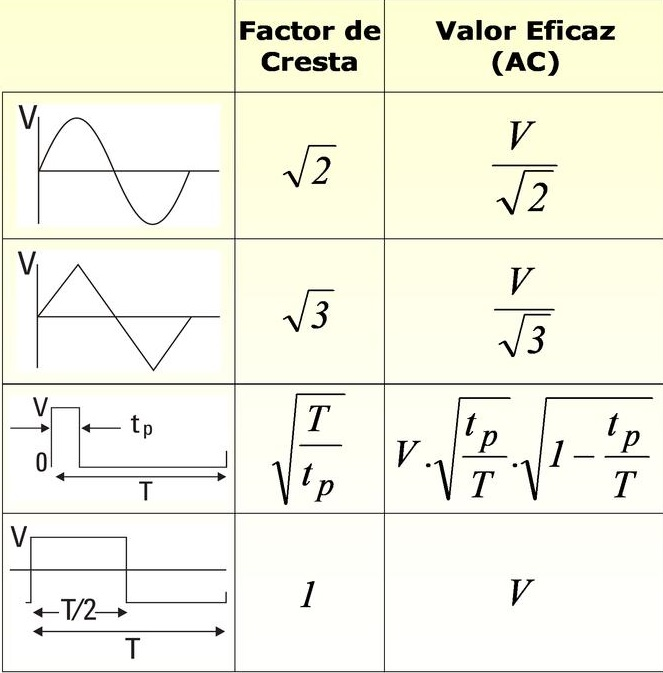
\includegraphics[width=0.4\linewidth]{Imagenes/FacCrest.jpg}
    \caption{Factores de Cresta de las señales más comunes}
    \label{fig:facCrest}
\end{figure}




%El propósito de este trabajo es justamente obtener en forma práctica dichas cotas para un determinado instrumento, comparando su respuesta con la de uno que usa detector de respuesta al valor eficaz verdadero, ya que, en principio, este tipo de voltímetro es capaz de medir cualquier forma de onda. 


